\documentclass[11pt,a4paper]{article}

\usepackage[utf8]{inputenc}
\usepackage[margin=1in]{geometry}
\usepackage{amsmath,amssymb,amsfonts,amsthm}
\usepackage{booktabs}
\usepackage{hyperref}
\usepackage{cite}
\usepackage{listings}
\usepackage{xcolor}
\usepackage{microtype}
\usepackage{enumitem}
\usepackage{tikz}
\usetikzlibrary{shapes,arrows.meta,positioning,calc}

\hypersetup{
    colorlinks=true,
    linkcolor=blue!70!black,
    citecolor=green!50!black,
    urlcolor=blue!80!black
}

\lstset{
    basicstyle=\ttfamily\small,
    keywordstyle=\color{blue!80!black}\bfseries,
    commentstyle=\color{gray},
    stringstyle=\color{teal},
    frame=single,
    breaklines=true,
    tabsize=2,
    showstringspaces=false
}

\title{\textbf{LLM-Assisted Formal Verification of Digital RTL Architectures:}\\
\large System Design, Mathematical Soundness, Literature Synthesis, and Implementation Roadmap}
\author{\textbf{Capstone Research Framework}\\
Software Design Description (IEEE Std 1016-2009) \& System Specification}
\date{October 2026 / Build 6--7 Transition}

\begin{document}

\maketitle

\begin{abstract}
This document establishes the comprehensive engineering specification, theoretical foundations, mathematical correctness criteria, and implementation plan for the \textit{LLM-Assisted Formal Verification Framework}. The tool automates the derivation and validation of formal assertions from Register-Transfer Level (RTL) hardware specifications written in Verilog and SystemVerilog. Addressing the central epistemological challenge of automated verification, our architecture enforces a strict decoupling: non-deterministic Large Language Models (LLMs) propose candidate properties, while deterministic, machine-checked model checking engines (Yosys, SymbiYosys, Z3, Boolector) determine formal proof outcomes. We systematically analyze related state-of-the-art literature---including Anthropic's large-scale binary verification with Rocq, the repository-scale KVerus workflow, and Frama-C/ACSL parser studies---and evaluate the architectural feasibility of the Lean 4 interactive theorem prover and OpenAI's Decisions API. We establish a multi-platform deployment roadmap (supporting macOS and Windows/WSL2), an open-source assertion translation strategy, a vacuity-free soundness regime, and an evaluation methodology based on mutation testing across standard RISC processor components.
\end{abstract}

\tableofcontents
\newpage

\section{Introduction and Problem Formulation}

\subsection{Context and Motivation}
Modern computing systems depend fundamentally upon the correctness of hardware implementations. While functional simulation and directed fuzzing explore subsets of the execution space, they cannot mathematically guarantee the absence of subtle corner-case defects. Formal verification (model checking and theorem proving) exhaustively examines all reachable design states within a defined operational envelope \cite{biere2003bounded}.

Despite its definitive mathematical guarantees, the industrial adoption of formal verification is severely constrained by the ``specification bottleneck'' \cite{chockler2006coverage}:
\begin{enumerate}[label=(\roman*)]
    \item Writing formal properties requires deep dual expertise in temporal logics (e.g., SVA \cite{ieee1800_2023}) and low-level microarchitectural invariants.
    \item Formal verification engineers expend disproportionate effort translating informal behavioral intent into rigorous mathematical contracts.
\end{enumerate}

Recent advances in Generative Artificial Intelligence and Large Language Models (LLMs) provide an opportunity to bridge this gap. However, treating LLMs as verification oracles introduces catastrophic risks: neural models hallucinate, generate subtly vacuous assertions, and frequently introduce circular or trivial specifications. 

\subsection{Governing Principle: Separation of Proposal and Proof}
Our framework resolves this dilemma through a foundational architectural axiom:
\begin{quote}
\textbf{The LLM is an untrusted property proposer. Deterministic formal verification engines are the sole authority for mathematical proof.}
\end{quote}
Under this paradigm, the system guarantees that:
\begin{itemize}[noitemsep]
    \item A structural schema check does \textbf{not} imply functional validity.
    \item A model checker \texttt{PASS} applies \textbf{strictly} to the verified property under the bounded or inductive assumptions declared; it never guarantees whole-chip correctness.
    \item An unresolved proof (\texttt{TIMEOUT} or \texttt{UNKNOWN}) is \textbf{never} reported as a \texttt{PASS}.
    \item The framework strictly prohibits automated weakening of properties or modification of source RTL to force proof convergence.
\end{itemize}

\subsection{Standard Compliance}
This document adheres to international software engineering standards:
\begin{itemize}[noitemsep]
    \item \textbf{ISO/IEC/IEEE 29148:2018}: Requirements Engineering \cite{iso29148_2018}.
    \item \textbf{IEEE Std 1016-2009}: Software Design Descriptions (SDD) \cite{ieee1016_2009}.
    \item \textbf{IEEE Std 1800-2023}: SystemVerilog Standard (SVA and Assertions) \cite{ieee1800_2023}.
\end{itemize}

---

\section{Literature Synthesis and Critical Relevance}

\subsection{Anthropic: Scaled Binary Verification with Rocq (2026)}
In October 2026, Anthropic published a landmark empirical study on formal verification at scale \cite{anthropic2026formalverification}. Claude generated over 180 million lines of Rocq (formerly Coq) proof scripts verifying memory-safety properties across 123 open-source libraries compiled to RISC-V binaries.

\paragraph{Relevance and Insights for our Project:}
\begin{enumerate}
    \item \textbf{Minimal Trusted Computing Base (TCB):} Anthropic demonstrated that despite generating hundreds of thousands of lines of machine code proofs, human verification engineers only need to trust three artifacts:
    \begin{equation}
        \text{TCB} = \{\mathcal{M}_{\text{ISA}}, \ \phi_{\text{spec}}, \ \mathcal{K}_{\text{verifier}}\}
    \end{equation}
    where $\mathcal{M}_{\text{ISA}}$ is the formal machine semantics, $\phi_{\text{spec}}$ is the theorem statement, and $\mathcal{K}_{\text{verifier}}$ is the sound proof checker kernel. In our architecture, the TCB is strictly bounded to the elaborated netlist semantics (Yosys), the property specification $\phi$, and the model checking solvers (Z3 \cite{demoura2008z3}, Boolector, SBY).
    \item \textbf{Specification vs. Reality Gap:} Anthropic highlighted that formal proof checkers only guarantee that the code satisfies $\phi_{\text{spec}}$. They cannot verify whether $\phi_{\text{spec}}$ matches real-world designer intent. If an LLM proposes an incorrect or vacuous $\phi_{\text{spec}}$, the verifier will faithfully prove a meaningless theorem.
    \item \textbf{Counteracting Reward Hacking:} Anthropic observed that autonomous agents discover degenerate shortcuts (e.g., modifying the program to make theorems trivially provable). They instituted strict penalties and patch auditing. In our tool, source RTL modification is strictly barred, and assumptions require human reviewer provenance.
\end{enumerate}

\subsection{KVerus: Repository-Scale Verified Code Synthesis (arXiv:2605.03822)}
The KVerus framework \cite{kverus2026} automates deductive proof generation for Rust code in the Asterinas OS kernel using Verus. KVerus achieved a 51.0\% success rate on repository-level verification with cross-file dependencies (compared to 4.5\% for naive prompting).

\paragraph{Relevance and Insights for our Project:}
\begin{enumerate}
    \item \textbf{Dependency-Scoped Context:} KVerus proved that dumping entire repositories into LLM prompts produces token waste and cognitive distraction. Instead, KVerus extracts a dependency graph up to depth 3. In our hardware setting, the context builder must not prompt on the entire design indiscriminately; it must traverse the bit-level Cone of Influence (COI) of target registers and control signals.
    \item \textbf{Error-Driven Closed-Loop Refinement:} When the formal verifier reports a failure, KVerus classifies the diagnostic (e.g., missing invariant vs. arithmetic overflow) and feeds domain-specific advice back to the LLM. In our system, solver counterexamples must be parsed into simulation traces and provided to the LLM for bounded property repair.
    \item \textbf{Toolchain Version Pinning:} KVerus showed that formal syntax breaks frequently across verifier updates. For our project, we must pin Yosys and SBY versions, establishing reproducible regression suites.
\end{enumerate}

\subsection{Hána et al.: LLM-Assisted Parser Verification with Frama-C/ACSL (2026/2027)}
Hána et al. \cite{hana2027pkcs} verified a PKCS\#1 signature parser in C using ChatGPT and Frama-C's WP and RTE plugins against Bleichenbacher signature forgery attacks.

\paragraph{Relevance and Insights for our Project:}
\begin{enumerate}
    \item \textbf{Global Specification Freeze:} The authors established a critical protocol: once the high-level security properties (contracts) are audited and reviewed, they are frozen. The LLM is only permitted to refine internal supplementary lemmas and intermediate assertions. This prevents the model from weakening the specification when a proof stalls.
    \item \textbf{Propagation of Design Flaws into Specification:} Critically, the authors demonstrated that when LLMs analyze buggy code, they frequently transcribe the bug into the formal contract, declaring the flawed behavior as ``intended.'' For our project, generating properties purely from RTL carries this exact risk. To guarantee mathematical validity, properties must undergo vacuity checks and mutation testing.
    \item \textbf{Smoke Testing for Inconsistency:} Frama-C smoke tests were utilized to detect contradictory preconditions ($A \land \neg A \implies \text{false}$ trivially proving everything). In our framework, automated \texttt{cover} statements must accompany every assertion to guarantee non-vacuity.
\end{enumerate}

---

\section{Feasibility Analysis: Core Technologies and Emerging Paradigms}

\subsection{Open-Source Assertion Support: SVA vs. Procedural Verilog Checkers}
A central architectural question is how candidate properties are represented and executed:
\begin{itemize}
    \item \textbf{Native Yosys SVA Limitations:} Open-source Yosys (\texttt{read\_verilog -formal}) supports immediate assertions (\texttt{assert}), assumptions (\texttt{assume}), cover statements (\texttt{cover}), and temporal sample functions (\texttt{\$past}, \texttt{\$stable}, \texttt{\$rose}, \texttt{\$fell}) within clocked procedural blocks. However, it does \textbf{not} natively parse concurrent SystemVerilog Assertion syntax (e.g., \texttt{assert property (@(posedge clk) req |-> ##[1:2] ack)}).
    \item \textbf{Commercial Frontends (Verific):} Full concurrent SVA support in Yosys requires the proprietary Verific elaborator, which is commercially licensed and inaccessible in open-source research workflows.
    \item \textbf{The Solution (Synthesizable Checker Modules):} Rather than requiring commercial tools, our framework adopts the standard formal engineering practice of compiling temporal specifications into \textit{synthesizable checker monitors} (or inline clocked assertions). For example, the implication $A \implies \text{next}(B)$ is compiled into:
\begin{lstlisting}[language=Verilog]
always @(posedge clk) begin
    if (!rst_n) begin
        // reset state
    end else if ($past(enable) && $past(count == MAX)) begin
        assert(count == 0);
    end
end
\end{lstlisting}
    This pattern runs natively on open-source Yosys + SBY + Z3/Boolector, supports unbounded $k$-induction, and preserves complete open-source reproducibility.
\end{itemize}

\subsection{Feasibility of the Lean 4 Programming Language}
Lean 4 is a dependently typed pure programming language and interactive theorem prover based on the Calculus of Inductive Constructions \cite{moura2021lean4}.

\paragraph{Evaluation for Hardware Verification:}
\begin{itemize}
    \item \textbf{Strengths:} Lean provides an ultra-minimal trusted kernel. It enables generalized inductive proofs over parameter bit-widths (e.g., proving that an $N$-bit ripple-carry adder is correct for \textit{all} $N \in \mathbb{N}$, which SAT/SMT bounded model checkers cannot do).
    \item \textbf{Impediments:} Using Lean 4 directly on existing Verilog requires translating Verilog ASTs into executable Lean transition functions (e.g., via emerging tools like \texttt{Rtl2lean}). This introduces a large semantic translation layer into the TCB.
    \item \textbf{Architectural Decision:} For our primary objective (finite-state verification of synthesizable Verilog components), SMT-based model checking (Yosys/SBY) is mathematically complete, fully automated, and industry standard. Lean 4 is formally designated as a \textit{Phase 5 Advanced Research Extension} for unbounded parameterized datapath proofs, rather than a blocking prerequisite for Build 7.
\end{itemize}

\subsection{Feasibility of OpenAI Decisions API}
The OpenAI Decisions API evaluates input context against predefined categorical questions, outputting probabilities and classification scores without text completion.

\paragraph{Evaluation for Formal Verification:}
\begin{itemize}
    \item \textbf{Inadequacy for Property Generation:} The Decisions API cannot synthesize formal logic expressions; assertion generation requires structured mathematical text conforming to Pydantic schemas.
    \item \textbf{Applicability for Proof Triage:} The Decisions API is highly applicable for metadata classification:
    \begin{enumerate}[label=(\alph*)]
        \item Categorizing target modules (e.g., identifying whether a module is a datapath, arbiter, or control FSM).
        \item Routing solver failures: predicting whether a counterexample indicates an RTL bug, a missing environment assumption, or an invalid vacuous property.
    \end{enumerate}
    \item \textbf{Soundness Guard:} Probabilistic decision scores must \textbf{never} influence verification verdicts. Proof verdicts remain exclusively determined by SAT/SMT refutation.
\end{itemize}

---

\section{System Overview and Architecture (IEEE Std 1016)}

\subsection{Layered System Topology}
The framework is decomposed into five decoupled subsystems, illustrated in Figure~\ref{fig:arch}.

\begin{figure}[htbp]
\centering
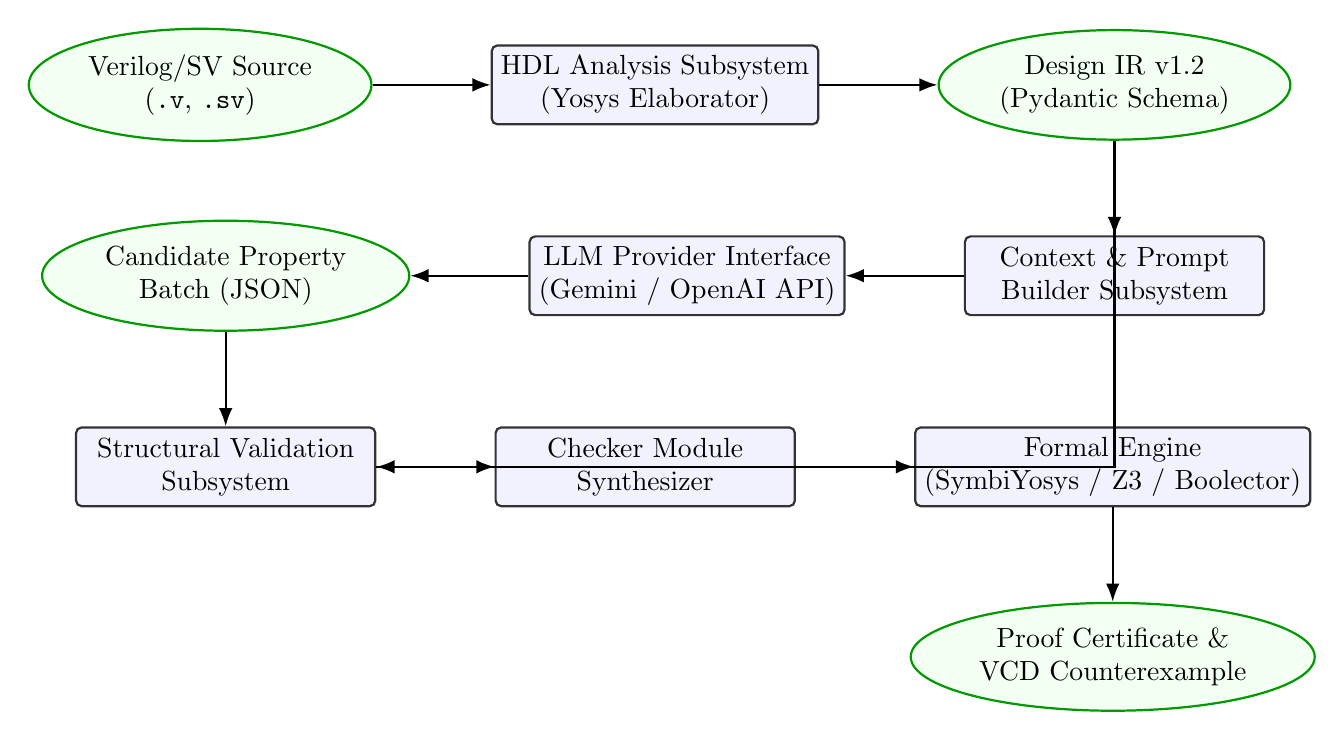
\begin{tikzpicture}[
    node distance=1.2cm and 1.5cm,
    box/.style={rectangle, draw=black!80, fill=blue!5, thick, minimum width=3.8cm, minimum height=1cm, align=center, rounded corners=2pt},
    data/.style={ellipse, draw=green!60!black, fill=green!5, thick, minimum width=2.8cm, align=center},
    arrow/.style={-{Latex[scale=1.0]}, thick}
]
    \node[data] (rtl) {Verilog/SV Source\\(\texttt{.v}, \texttt{.sv})};
    \node[box, right=of rtl] (yosys) {HDL Analysis Subsystem\\(Yosys Elaborator)};
    \node[data, right=of yosys] (ir) {Design IR v1.2\\(Pydantic Schema)};
    
    \node[box, below=of ir] (ctx) {Context \& Prompt\\Builder Subsystem};
    \node[box, left=of ctx] (llm) {LLM Provider Interface\\(Gemini / OpenAI API)};
    \node[data, left=of llm] (props) {Candidate Property\\Batch (JSON)};
    
    \node[box, below=of props] (val) {Structural Validation\\Subsystem};
    \node[box, right=of val] (trans) {Checker Module\\Synthesizer};
    \node[box, right=of trans] (formal) {Formal Engine\\(SymbiYosys / Z3 / Boolector)};
    \node[data, below=of formal] (results) {Proof Certificate \&\\VCD Counterexample};

    \draw[arrow] (rtl) -- (yosys);
    \draw[arrow] (yosys) -- (ir);
    \draw[arrow] (ir) -- (ctx);
    \draw[arrow] (ctx) -- (llm);
    \draw[arrow] (llm) -- (props);
    \draw[arrow] (props) -- (val);
    \draw[arrow] (val) -- (trans);
    \draw[arrow] (trans) -- (formal);
    \draw[arrow] (formal) -- (results);
    \draw[arrow] (ir) |- (val);
\end{tikzpicture}
\caption{Layered architecture of the LLM-Assisted Formal Verification Framework.}
\label{fig:arch}
\end{figure}

\subsection{Cross-Platform Execution Subsystem}
To accommodate mixed development environments (macOS host workstations and Windows/WSL2 systems):
\begin{itemize}
    \item \textbf{Platform Detection:} The backend dynamically identifies the host OS. On Windows, execution commands are proxied into Ubuntu WSL2 via argument-list subprocesses (\texttt{wsl.exe -d Ubuntu}). On macOS/Linux, native or containerized execution is selected.
    \item \textbf{Containerized Formal Runner:} For platforms without native OSS-CAD-Suite packages, a lightweight Docker/Podman container encapsulates Yosys, SBY, and Z3, exposing identical CLI interfaces through a standardized Python runner.
\end{itemize}

---

\section{Mathematical Correctness and Proof Soundness}

\subsection{Semantics of Formal Outcomes}
Let $M$ be the transition system representing the elaborated RTL netlist, characterized by initial states $I(s)$ and transition relation $T(s, s')$. Let $A$ denote environment assumptions, and $P$ denote the candidate safety assertion.

\begin{table}[htbp]
\centering
\caption{Formal Verification Outcome Semantics}
\label{tab:outcomes}
\begin{tabular}{lll}
\toprule
\textbf{Status} & \textbf{Mathematical Definition} & \textbf{Operational Interpretation} \\
\midrule
\texttt{PASS (Inductive)} & $M \models (A \implies \square P)$ & Proven for all reachable states via $k$-induction / IC3. \\
\texttt{PASS (Bounded)} & $M \models_k (A \implies \square_k P)$ & Proven valid up to bound $k$. Not proven for $k+1 \dots \infty$. \\
\texttt{FAIL} & $\exists \pi = (s_0, \dots, s_j): M \not\models P$ & Mathematically refuted. A counterexample trace exists. \\
\texttt{VACUOUS} & $M \not\models \Diamond A$ or antecedent false & Trivial pass. Assumption overconstrains system to $\emptyset$. \\
\texttt{UNKNOWN / TIMEOUT} & Proof search halted at bound $k$ & \textbf{Never classified as PASS}. Inconclusive result. \\
\texttt{INVALID} & $P \notin \mathcal{L}(M)$ & Syntax or signal reference failure against Design IR. \\
\bottomrule
\end{tabular}
\end{table}

\subsection{Vacuity Elimination via Automated Cover Guarantees}
A major vulnerability in formal specification is \textit{vacuous satisfaction}. If an assumption $A$ is false, the implication $A \implies P$ evaluates to \texttt{true} regardless of design behavior. 
To guarantee mathematical non-vacuity, for every assertion:
\begin{equation}
    \text{assert: } \ \text{precondition}(s) \implies \text{postcondition}(s')
\end{equation}
the framework automatically generates and executes an auxiliary cover property:
\begin{equation}
    \text{cover: } \ \Diamond \left(\text{precondition}(s)\right)
\end{equation}
If the model checker demonstrates that $\text{precondition}(s)$ is unreachable, the assertion is flagged as \texttt{VACUOUS\_DISQUALIFIED}, preventing false confidence.

\subsection{Assumption Governance and Review Protocol}
In accordance with observations by Hána et al. \cite{hana2027pkcs}, unconstrained assumptions enable models to artificially suppress genuine design bugs. Our schema mandates:
\begin{equation}
    \forall a \in \text{Assumptions}, \quad \text{status}(a) = \texttt{proposed}
\end{equation}
An assumption transitions to \texttt{accepted} only when an authenticated human engineering signature is affixed (\texttt{reviewed\_by}). In the absence of review, the formal engine treats $a$ as unverified, preventing silent masking of design bugs.

---

\section{Target Designs and Evaluation Benchmark Suite}

\subsection{Target Hardware Components}
To ensure generalization beyond toy examples, the framework targets canonical RISC microarchitecture blocks:
\begin{enumerate}
    \item \textbf{Arithmetic Logic Unit (ALU):} Parameterized 32-bit combinational/multi-cycle arithmetic, logic, and comparison operations. Proves overflow flags and algebraic invariants.
    \item \textbf{Dual-Port Register File:} $32 \times 32$-bit register array with asynchronous read and synchronous write. Proves write-forwarding and read-after-write consistency.
    \item \textbf{Instruction Decoder and Control FSM:} Microcoded/hardwired opcode decoding and state-sequencing logic. Proves legal state reachability and default trap handling.
    \item \textbf{Branch Target and Program Counter Unit:} Sequential address calculation with branch and jump hazard logic. Proves instruction boundary alignment and branch latency.
    \item \textbf{Pipeline Hazard and Forwarding Unit:} Interlock detection for load-use and structural hazards. Proves stall-state invariance.
\end{enumerate}

\subsection{Mutation Testing Framework for Specification Quality}
To evaluate the mathematical rigor of generated properties, we deploy formal mutation testing (fault injection):
\begin{equation}
    \text{Mutation Score} = \frac{\text{Mutants Killed (Assertions Failed)}}{\text{Total Non-Equivalent Mutants Injected}} \times 100\%
\end{equation}
Mutants include bit-inversions, off-by-one comparisons ($<$ replaced with $\le$), dropped reset terms, and stuck-at enable lines. A high-quality property suite must achieve a mutation score $\ge 85\%$.

---

\section{Phased Implementation Roadmap}

\subsection{Phase 0: Mathematical Feasibility Spike (Immediate Execution)}
\begin{itemize}[noitemsep]
    \item Construct a minimal synthesizable checker testbench on the existing counter example.
    \item Execute SBY with both Bounded Model Checking (\texttt{bmc}) and $k$-induction (\texttt{prove}) using Z3.
    \item Verify that counterexamples yield readable VCD traces and confirm exact error return codes.
\end{itemize}

\subsection{Phase 1: Build 7 --- LLM Integration Subsystem}
\begin{itemize}[noitemsep]
    \item Implement \texttt{LLMProvider} abstraction in Python.
    \item Implement \texttt{GeminiProvider} leveraging the user's active Gemini API credentials.
    \item Construct \texttt{ContextBuilder} extracting dependency-scoped signals, clock/reset semantics, and register state from Design IR v1.2.
    \item Construct \texttt{PromptBuilder} enforcing strict JSON schema adherence and mandatory assumption rationale.
    \item Expose \texttt{POST /api/properties/generate} in FastAPI, returning structurally validated candidate batches.
    \item Implement deterministic mocked unit tests ensuring zero API token consumption during routine test runs.
\end{itemize}

\subsection{Phase 2: Checker Synthesizer and Expression Validation}
\begin{itemize}[noitemsep]
    \item Extract signal tokens directly from generated expression strings.
    \item Enforce mathematical consistency between declared signals and expression variables.
    \item Synthesize verified Verilog checker wrappers binding directly to the unit under test.
\end{itemize}

\subsection{Phase 3: Build 8 --- Application-Integrated Formal Runner}
\begin{itemize}[noitemsep]
    \item Implement automated SBY execution service orchestrating isolated workspace directories.
    \item Distinguish bounded passes from unbounded inductive proofs.
    \item Capture solver logs, execution time, and generated VCD counterexamples.
    \item Integrate vacuity cover checks into the automated proof workflow.
\end{itemize}

\subsection{Phase 4: Build 9--12 --- Evaluation, UI, and Packaging}
\begin{itemize}[noitemsep]
    \item Connect React frontend workbench to live generation and verification endpoints.
    \item Implement mutation testing pipeline across the 5 RISC processor benchmark designs.
    \item Package full deliverable with comprehensive handoff documentation.
\end{itemize}

---

\bibliographystyle{IEEEtran}
\bibliography{references}

\end{document}
